\documentclass[12pt,a4paper,oneside]{article}

\usepackage[pdftex,
            pdfauthor={Albert Zak},
            pdftitle={Dynamic Software Updating in Erlang/OTP},
            pdfsubject={Bachelor Thesis},
            hidelinks,
            driverfallback=hypertex]{hyperref}
\usepackage[english]{babel}
\usepackage{lmodern}
\usepackage[utf8]{inputenc}
\usepackage[T1]{fontenc}
% \usepackage{arialu}
% \renewcommand{\familydefault}{\sfdefault}
% \normalfont
\renewcommand{\rmdefault}{phv} % Arial
\renewcommand{\sfdefault}{phv} % Arial

\usepackage{microtype}
\usepackage{geometry}
\usepackage{bookmark}
\usepackage{listings}
\usepackage[inline]{enumitem}
\usepackage{subcaption}
\usepackage{tabularx}
\usepackage{multirow}
\usepackage{floatrow, makecell}
\usepackage{hhline}
\usepackage{boldline}
\usepackage{algpseudocode}
\usepackage{stackengine}
\usepackage{tikz}
\usetikzlibrary{trees,arrows,fit,positioning,shapes.geometric,shadows}
\PassOptionsToPackage{usenames,dvipsnames,svgnames,table}{xcolor}
\usepackage{xcolor-solarized}
\usepackage{gitdags}
\usepackage[singlespacing]{setspace}
\usepackage[acronym,nopostdot,style=super,nonumberlist,nogroupskip]{glossaries}
\usepackage{fancyhdr}
\usepackage{hyphenat}
\hyphenation{name-space}
\usepackage{forest}
\forestset{
  dir tree/.style={
    for tree={
      parent anchor=south west,
      child anchor=west,
      anchor=mid west,
      inner ysep=-3pt,
      grow'=0,
      align=left,
      edge path={
        \noexpand\path [draw, very thin, lightgray, \forestoption{edge}] (!u.parent anchor) ++(1em,0) |- (.child anchor)\forestoption{edge label};
      },
      font=\ttfamily,
      if n children=0{}{
        delay={
          prepend={[,phantom, calign with current]}
        }
      },
      fit=band,
      before computing xy={
        l=2em
      }
    },
  }
}

\pagestyle{fancy}
\fancyhf{}
\cfoot{\thepage}
\renewcommand{\headrulewidth}{0pt}

\makeglossaries{}
\newacronym{bif}{BIF}{Built-in Function}
\newacronym{erts}{ERTS}{Erlang Run-Time System}
\newacronym{vm}{VM}{Virtual Machine}
\newacronym{otp}{OTP}{Open Telecom Platform}
\newacronym{sasl}{SASL}{System Architecture Support Libraries}
\newacronym{os}{OS}{Operating System}
\newacronym{vcs}{VCS}{Version Control System}
\newacronym{api}{API}{Application Programming Interface}
\newacronym{ci}{CI}{Continuous Integration}
\newacronym{cli}{CLI}{Command Line Interface}
\newacronym{ram}{RAM}{Random Access Memory}
\newacronym{dsu}{DSU}{Dynamic Software Updating}
\newacronym{tls}{TLS}{Transport Layer Security}
\newacronym{http}{HTTP}{Hypertext Transfer Protocol}
\newacronym{lxc}{LXC}{Linux Containers}
\newacronym{beam}{BEAM}{Bogdan/Björn's Erlang Abstract Machine}
\newacronym{ecs}{ECS}{Elastic Compute Cloud Container Service}
\newacronym{cow}{CoW}{Copy-on-Write}
\newacronym{appup}{appup}{Application Upgrade Instructions}
\newacronym{relup}{relup}{Release Upgrade Instructions}
\newacronym{tmpfs}{tmpfs}{Temporary File System}
\newacronym{nif}{NIF}{Native Implemented Functions}
\newacronym{rest}{REST}{Representational State Transfer}
\newacronym{etf}{ETF}{Erlang External Term Format}
\newacronym{ssh}{SSH}{Secure Shell}
\newacronym{mfa}{MFA}{Module, Function, Arity}
\newacronym{sse}{SSE}{Server-Sent Events}
\newacronym{ip}{IP}{Internet Protocol}
\newacronym{url}{URL}{Uniform Resource Locator}
\newacronym{cd}{CD}{Continuous Delivery}
\newacronym{hipe}{HiPE}{High Performance Erlang}
\newacronym{paas}{PaaS}{Platform as a Service}


\lstset{
  language=bash,
  numbers=left,
  numberstyle=\small\color{lightgray},
  basicstyle=\ttfamily,
  frame=tb,
  firstnumber=0,
  stepnumber=5
}
% Hide number in first line of code listings
\makeatletter
\def\lst@PlaceNumber{\ifnum\value{lstnumber}=0\else
  \rlap{\normalfont\kern\linewidth \kern\lst@numbersep\lst@numberstyle{\thelstnumber}}\fi}
\makeatother

\pdfpageheight=297mm
\pdfpagewidth=210mm
\geometry{a4paper, left=30mm, right=25mm, top=30mm, bottom=30mm}

\begin{document}

\frenchspacing

\pagestyle{empty}
\thispagestyle{empty}
\begin{picture}(50,50)
  \put(-70,40){\hbox{
\includegraphics[width=5cm]{fhcw-logo.pdf}}}
\end{picture}

\vspace*{-5.8cm}


\begin{center}
  \vspace{6.5cm}
  \hspace*{-1.0cm} {\LARGE \textbf{Deployment of Erlang/OTP Releases\\}}
  \hspace*{-1.0cm} {\LARGE \textbf{via Dynamic Software Updating\\}}
  \vspace{0.5cm}
  \hspace*{-1.0cm} Implementation of a Node Agent, and Analysis of Failure Modes \\

  \vspace{2cm}

  \hspace*{-1.0cm} {\LARGE \textbf{Bachelor Thesis\\}}
  \vspace{0.65cm}

  \hspace*{-1.0cm} Submitted in partial fulfillment of the requirements for the degree of \\

  \vspace{0.65cm}

  \hspace*{-1.0cm} \textbf{Bachelor of Science in Engineering} \\
  \vspace{0.65cm}
  \hspace*{-1.0cm} to the University of Applied Sciences FH Campus Wien \\
  \vspace{0.4cm}
  \hspace*{-1.0cm} Bachelor Degree Program\\
  \vspace{0.4cm}
  \hspace*{-1.0cm} Information Technology and Telecommunications\\

  \vspace{2cm}

  \hspace*{-1.0cm} \textbf{Author:} \\
  \vspace{0.2cm}
  \hspace*{-1.0cm} Albert Zak \\
  \vspace{0.7cm}

  \hspace*{-1.0cm} \textbf{Student identification number:}  \\
  \vspace{0.2cm}
  \hspace*{-1.0cm} 1510475069 \\
  \vspace{0.7cm}

  \hspace*{-1.0cm} \textbf{Supervisor:} \\
  \vspace{0.2cm}
  \hspace*{-1.0cm} Priv.-Doz. Mag.rer.soc.oec.\\
  \hspace*{-1.0cm} Dipl.-Ing. Dipl.-Ing. Dr.techn.\\
  \hspace*{-1.0cm} Karl Michael Göschka \\
  \vspace{0.7cm}

  \hspace*{-1.0cm} \textbf{Date:} \\
  \vspace{0.2cm}
  \hspace*{-1.0cm} 01.06.2018 \\

\end{center}

\newpage

\vspace*{16cm}
\begin{flushleft}
  \underline{Declaration of authorship:}\\
  \vspace{0.5cm}
  I declare that this Bachelor Thesis has been written by myself. I have not used any other than the listed sources, nor have I received any unauthorized help.\\
  \vspace{0.5cm}
  I hereby certify that I have not submitted this Bachelor Thesis in any form (to a reviewer for assessment) either in Austria or abroad.\\
  \vspace{0.5cm}
  Furthermore, I assure that the (printed and electronic) copies I have submitted are identical.\\
  \vspace{1cm}
  Date: \hspace{5.3cm} Signature:
\end{flushleft}


\newpage
\pagestyle{fancy}
\pagenumbering{roman}
\cleardoublepage{}

\section*{Abstract}

Erlang/\acrshort{otp} is a programming language and runtime system for building distributed systems with high availability requirements. The Erlang/\acrshort{otp} release process is at odds with the practice of \acrlong{ci}, as assembling a release capable of \acrfull{dsu} requires manual interaction at many steps. Previous work on automating Erlang/\acrshort{otp} Release generation has addressed parts of the process by abstracting the low-level mechanics of the build step, but tasks such as versioning and handling artifacts were left to the developer. This thesis presents a release generation tool designed for hands-off operation as part of a Continuous Integration pipeline. Tight coupling with Git allows reliable identification of releases by discarding numeric versions in favor of commit hashes, and a centralized release store takes care of handling artifacts. Evaluation of a reference implementation on six hosted Continuous Integration providers (\emph{CircleCI, Codeship, Semaphore, Shippable, Travis CI,} and \emph{Wercker}) demonstrates comparable run time and ease of setup.


\renewcommand{\glsnamefont}[1]{\textbf{#1}}
\doublespacing
\printglossary[title=List of Abbreviations,nonumberlist,type=\acronymtype]
\singlespacing

\cleardoublepage

\section*{Key Terms}
Continuous Delivery\\
Git \\
Tooling \\
Erlang \\
Elixir \\
Automation \\
Dynamic Software Updating \\

\cleardoublepage

\tableofcontents{}

\cleardoublepage

\pagenumbering{arabic}

\section{Introduction}

The contributions of this work are \begin{enumerate*}[label=(\roman*)]
  \item an extension to the pipeline described in~\cite{zak18} to bootstrap an Erlang/\acrshort{otp} (\emph{\acrlong{otp}}) node with a single command, which pulls artifacts from a central store and deploys them without interaction; and
  \item an analysis of possible failure modes and root causes that may prevent an upgrade from being applied successfully via \acrfull{dsu}.
\end{enumerate*} This section explains relevant terminology and shows where manual interaction is required to deploy \acrshort{otp} Releases.

\subsection{Erlang/OTP}

Erlang is a programming language for building concurrent, distributed systems with high availability requirements. Initially designed by Ericsson for telephone exchanges, it has been embraced by industries with similar needs: finance, gaming, betting, messaging, middleware, and databases. Development of Erlang took place starting in 1986 at the Ericsson Computer Science Laboratory, and in 1998 Erlang was released as Open Source.~\cite{armstrong2007history}

\acrshort{otp} stands for \acrlong{otp}, and is a combination of library applications, design patterns, conventions, and documentation. Erlang is almost always used in conjunction with \acrshort{otp}, hence the name Erlang/\acrshort{otp}.~\cite{ferd}

The language is often described as functional, although it is not strictly side effect free or referentially transparent. Erlang compiles to bytecode, which is executed by a \acrfull{vm}. The current Erlang \acrshort{vm} – the \emph{\acrshort{beam}}, short for \emph{\acrlong{beam}} – is written in C and supports various machine architectures. Multiple languages that compile to \acrshort{beam} bytecode have been created, most famously \emph{Elixir} and \emph{Lisp Flavored Erlang}. Actor model processes are the language's concurrency primitives: Functions can be spawned to create lightweight \acrshort{beam} processes. They are different from \acrfull{os} processes or threads, being preemptively scheduled by the \acrshort{beam}. Erlang/\acrshort{otp} systems commonly ``run millions of processes simultaneously [with each one taking] less than a kilobyte of space.''~\cite{larson}

\paragraph{\acrshort{otp} Applications.}
Erlang code is constructed out of functions defined within \mbox{\emph{module}} files bearing an \lstinline|*.erl| extension. \emph{\acrshort{otp} Applications} group related modules into reusable units to provide well-defined start and stop semantics, including an \emph{application resource file} (\lstinline|*.app|) containing additional metadata such as a version string and a list of other applications that this application depends on, and which need to be started beforehand. Every application has a dependency on at least \lstinline|kernel| and \lstinline|stdlib|, and both must be specified in the application resource file.~\cite{doc:otp}

\acrshort{otp} also enforces a certain directory structure for applications.~\cite{logan:otp}

\paragraph{\acrshort{otp} Releases.} Whole projects consisting of multiple applications are packaged and deployed as \acrshort{otp} Releases. They are described by a release resource (\lstinline|*.rel|) file, which specifies additional metadata, such as a version string for the entire release, the included version of the \emph{\acrlong{erts}} (\acrshort{erts}), and a list of applications with their respective version strings that comprise the release.

From this release resource file, various tools can be used to create a boot script and assemble the release into a single compressed tarball (\lstinline|*.tar.gz|) package.~\cite{doc:otp} A packaged release contains everything necessary to bootstrap an \emph{embedded target system} on another machine, also called a \emph{node}. Depending on the tool used to generate the release, it may include additional convenience scripts to upgrade or inspect the target system.

\paragraph{\acrlong{dsu}.} A core feature of Erlang is its support for \acrfull{dsu}, also referred to as on-the-fly upgrading, or hot code loading. The \acrshort{beam} keeps up to two versions of a module loaded in memory, and both versions of the code may run side by side.~\cite{cesarini:otp} \acrshort{otp} provides generic \emph{behaviours} that \emph{callback modules} can implement to normalize start, stop and upgrade semantics, among others.~\cite{doc:otp} Erlang systems constructed according to \acrshort{otp} patterns, grouped into \acrshort{otp} Applications, and packaged as \acrshort{otp} Releases enjoy additional support for \acrshort{dsu} via instruction files: \emph{\acrshort{appup}s} (\emph{\acrlong{appup}}) and \emph{\acrshort{relup}s} (\emph{\acrlong{relup}}).

First, there are high-level, often handwritten \acrfull{appup} files, one for each \acrshort{otp} Application. These files are fed into release generation tools where they are translated and combined into a single low-level \acrshort{relup} file, thus making a given release \acrshort{dsu}-capable.~\cite{doc:otp} The \acrshort{relup} file contains instructions on how to upgrade a node running a previous version. A single release package can include one \acrshort{relup} file which may know how to upgrade from multiple previous releases. These files also contain instructions on how to downgrade to the previous version in case the upgrade fails.~\cite{doc:otp}

\subsection{Problem}\label{sec:problem} Most existing release generation tools require manual interaction at various steps, and are generally not trivial to set up and use out of the box in a noninteractive build environment, such as a \acrfull{ci} pipeline. Additionally, there are some pitfalls when developers assemble releases on, for example, their \emph{macOS} development machines and then attempt to start them on \emph{Linux} in production~\cite{cesarini:otp}: This fails with a nonobvious error. To generate an \acrshort{otp} Release capable of \acrshort{dsu}, a developer needs to manually write \acrshort{appup} files and increment version numbers for all changed applications. The \acrshort{otp} Release resource file has an additional, separate version number that needs to be updated between commits to be able to perform \acrshort{dsu}. Then, to generate upgrade instructions, previous releases need to be fetched and unpacked. Lastly, the developer has to invoke various commands to assemble the final release package tarball.~\cite{ferd}

This process is tedious to perform manually, and impedes frequent deployment of small changes. Likewise, complex code changes are more likely to fail when applied via \acrshort{dsu}.~\cite{hicks} The unfortunate consequence is that developers are discouraged from using Erlang's \acrshort{dsu} capabilities unless absolutely necessary.~\cite{ferd}

\subsection{Contribution}

This work contributes design, implementation and evaluation of an extension to the build tool described in~\cite{zak18} for deploying Erlang/\acrshort{otp} Releases with support for \acrshort{dsu}. Its aim is to run without user interaction and to require as little configuration as possible. Additionally, the evaluation includes an analysis of \acrshort{dsu} failure modes.

\paragraph{Goal.} The goal is to develop a prototype implementation for bootstrapping an Erlang node with a single command. The node agent subscribes to the previously described release store to fetch release packages, download, extract, and deploy them; as well as apply \acrshort{dsu} instructions.

\paragraph{Method.} The thesis describes the architectural and design decisions made while iteratively implementing said node agent. The prototype is then used to tests the boundaries of the \acrshort{dsu} process. Finally, the work discusses limitations and advantages of the implementation.

\cleardoublepage
\subsection{State of the Art}\label{sec:sota}

The proposed tool, \emph{BeamUp}, relies on several layers of existing tooling, as visualized in Figure~\ref{fig:tools}. At the lowest level, Erlang/\acrshort{otp} ships with the \acrfull{sasl} that include the two basic building blocks for \acrshort{dsu} support: \lstinline|systools| provides low-level functions for \emph{offline} release generation, and \lstinline|release_handler| is used to perform an \emph{online} hot upgrade of a running node.~\cite{doc:otp}
Elixir projects are built with \lstinline|mix| (not pictured) and releases are generated with \lstinline|distillery|~\cite{distillery}, which handles generation of upgrade instructions itself, and directly interacts with \lstinline|systools|. Erlang projects, however, need more coaxing: Modules and dependencies are compiled with \lstinline|rebar3|, \acrfull{appup} files are generated on a best-effort basis by comparing \acrshort{beam} bytecode via a plugin to \lstinline|rebar3|~\cite{rebar3appup}, while release assembly is done by another intermediary tool, \lstinline|relx|~\cite{loder2016production}.

\vspace{2cm}
\begin{figure}[h]
  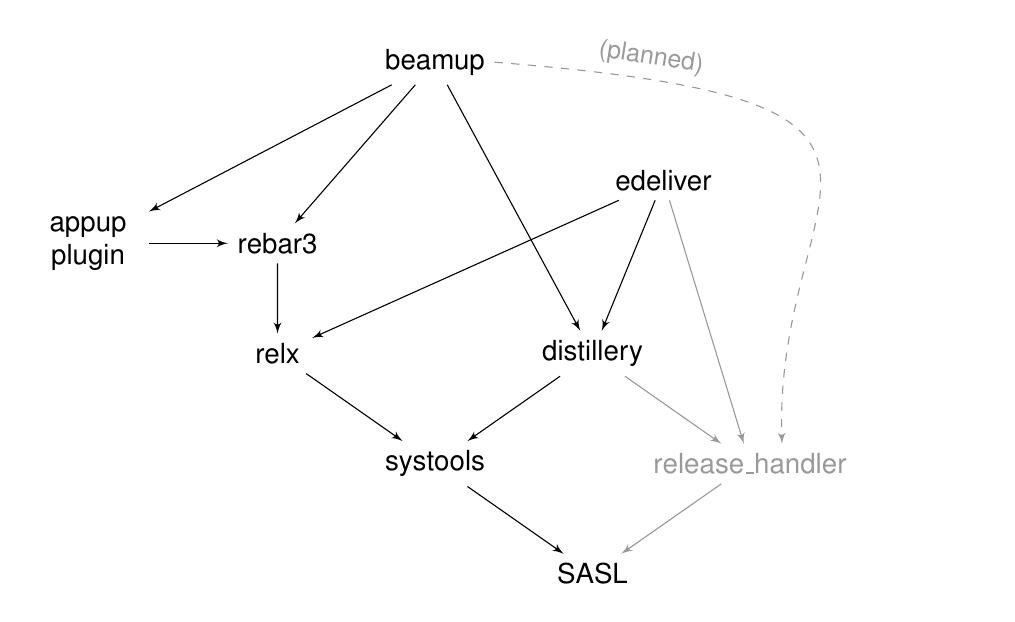
\begin{tikzpicture}[sibling distance=40mm,
    level distance=14mm,edge from parent,>=latex']
    \tikzstyle{edge from parent}=[draw,<-]
    \node (edeliver) at (0.9, 5) {\lstinline|edeliver|};
    \node (beamup) at (-2, 6.5) {\lstinline|beamup|};

    \node {\lstinline|SASL|} [grow'=up] {
      child {node {\lstinline|systools|}
        child {node (relx) {\lstinline|relx|}
          child {node (rebar3) {\lstinline|rebar3|}}}
        child {node (distillery) {\lstinline|distillery|}}}
      child {node (release_handler) [text=black!40] {\lstinline|release_handler|} edge from parent[draw=black!40]}
    };

    \node (appup) [left=10mm of rebar3,text centered,text width=13mm] {\lstinline|appup| \lstinline|plugin|};

    \draw[->] (appup) -- (rebar3);

    \draw[->] (edeliver) -- (distillery);
    \draw[->] (edeliver) -- (relx);
    \draw[->,draw=black!40] (edeliver) -- (release_handler);
    \draw[->,draw=black!40] (distillery) -- (release_handler);

    \draw[->] (beamup) -- (distillery);
    \draw[->] (beamup) -- (rebar3);
    \draw[->] (beamup) -- (appup);
    \draw[->,dashed,draw=black!40] (beamup.east) .. controls (5,6) and (2.3,5) .. node[very near start,sloped,above,text=black!40] {\small{(planned)}} (release_handler.32);

  \end{tikzpicture}
  \caption{Dependencies between selected tools to create and handle releases.}\label{fig:tools}
\end{figure}

\cleardoublepage
\section{Related Work}\label{sec:related_work}

There have been several attempts to automate Erlang/\acrshort{otp} deployment.

\emph{Edeliver}~\cite{edeliver,talk:edeliver} shares very similar goals to the proposed tool. It supports Erlang and Elixir projects, coaxing any of the following tools used on a project: \lstinline|rebar|, \lstinline|relx|, \lstinline|exrm|, or \lstinline|distillery|. It generates releases capable of \acrshort{dsu} with configurable autogenerated version strings. To provide a repeatable build environment, Edeliver opens a \acrfull{ssh} tunnel to a separate build host and assembles the release remotely. Written in \lstinline|bash|, it has no additional dependencies. The tool also handles deployment via \acrshort{ssh}, including remotely performing \acrshort{dsu}.

A different approach to release assembling relies on \emph{Nix}, a general purpose package manager borrowing ideas from functional programming: immutability, pure functions, and referential transparency.~\cite{nix1} Its artifacts are identified via cryptographic hashes of all inputs used to build them. Nix provides repeatable environments to build packages in, similar to what containers are used for in this work, but with stronger determinism. Nix forms the base of \emph{NixOS}~\cite{nixos}, a full featured Linux distribution where almost all components are controlled by Nix via symbolic links.

Previous work by~\cite{erlangnix} allows dependencies of Erlang/\acrshort{otp} projects to be managed via Nix, relying on \cite{hex2nix} to provide Nix metadata, called \emph{Expressions}, for most of the Erlang and Elixir packages hosted on \lstinline|hex.pm|, the primary package repository of the Erlang/\acrshort{otp} ecosystem. Lastly,~\cite{erlangnix2}~presents a pipeline to deploy Erlang/\acrshort{otp} projects using Nix.

\section{Implementation}

The contribution of this work, the tool \emph{BeamUp}, is implemented in three parts. First, the \emph{\acrlong{cli}} (\emph{\acrshort{cli}}) tool takes care of setting up a clean environment for the build to run in. Second, the \emph{builder} performs the  steps to assemble an artifact. To generate \acrshort{dsu} instruction files, the builder needs to fetch previous artifacts from a central location. The third component, the \emph{store}, manages the life cycle of artifacts.

\begin{figure}[h]
  \centering
  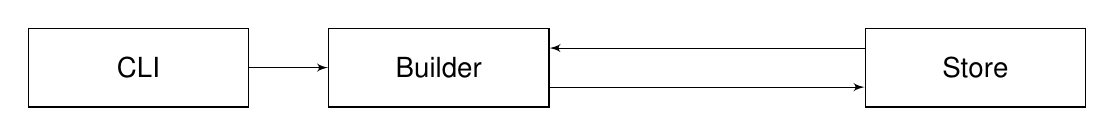
\begin{tikzpicture}[>=latex']
    \tikzset{block/.style={
      draw,
      rectangle,
      align=center,
      minimum width=2.8cm,
      minimum height=1cm
    }};

    \node [block] (cli) {CLI};
    \node [block, right=1cm of cli] (builder) {Builder};
    \node [block, right=4cm of builder] (store) {Store};

    \path[draw,->] (cli) edge (builder);
    \path[draw,<-] (builder.10) -- (store.170);
    \path[draw,->] (builder.350) -- (store.190);

  \end{tikzpicture}
  \caption{Architecture outline.}\label{fig:impl}
\end{figure}

\subsection{\acrlong{cli} Tool}

The main point of entry to the \acrshort{cli} tool is the \emph{launcher}. Acting as the starting point for all invocations, it is implemented as a \lstinline|bash| script. To provide a repeatable build environment, the launcher prefers to start a well-known \emph{Docker} container to run the given command in (see figure~\ref{fig:cliseq}). If, however, the launcher is invoked as part of an already running \acrshort{ci} container, it is not possible to start a new one. Thus, the launcher first has to detect whether it is running inside a container or not. In case it is being called directly on a host or a \acrfull{vm}, and is able to start containers, the launcher pulls the correct image for the host's machine architecture in combination with the requested Erlang/OTP version. Then it sets up volume mounts and environment variables, and calls the Docker client to start the container.

If the launcher is already running inside a container, the responsibility is reduced to passing the given arguments through to the \emph{container entrypoint}. The following paragraphs describe how each component of the launch sequence, including installation of the \acrshort{cli} tool itself, is implemented.

\begin{figure}[h]
  \centering
  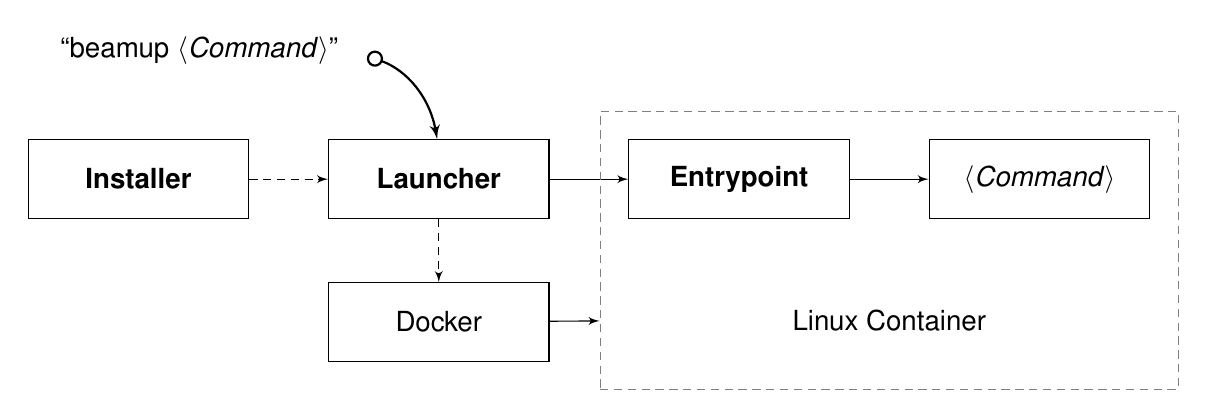
\begin{tikzpicture}[>=latex']
    \tikzset{block/.style={
      draw,
      rectangle,
      align=center,
      minimum width=2.8cm,
      minimum height=1cm
    }};

    \node [block] (installer) {\textbf{Installer}};
    \node [block, right=1cm of installer] (launcher) {\textbf{Launcher}};
    \node [block, right=1cm of launcher] (entrypoint) {\textbf{Entrypoint}};
    \node [block, right=1cm of entrypoint] (command) {$\langle$\emph{Command}$\rangle$};
    \node [block, below=0.8cm of launcher] (docker) {Docker};

    \node [inner sep=0pt,
      yshift=-1.8cm,
      minimum height=0.6cm,
      fit={(entrypoint) (command)},
      label=center:Linux Container] (container) {};

    \node [
      above left=1cm and -0.5cm of launcher,
      label=left:\text{``\lstinline|beamup| $\langle$\emph{Command}$\rangle$}''] (start) {};

    \path[draw,->] (launcher) edge (entrypoint)
      (entrypoint) edge (command);

    \path[densely dashed,->] (installer) edge (launcher)
      (launcher) edge (docker);

    \path[draw,o->,thick] (start) edge[bend left] (launcher);

    \node [draw=black!50, densely dashed, fit={
      (entrypoint) (command) (container)
    }, inner sep=10pt] (container_box) {};

    \path[draw,->] (docker) edge (container -|container_box.west);

  \end{tikzpicture}
  \caption{\acrshort{cli} execution sequence.}\label{fig:cliseq}
\end{figure}

\cleardoublepage
\paragraph{Installation.} The \acrshort{cli} tool is installed by downloading a \lstinline|bash| script and piping it to the shell (Listing~\ref{lst:curlpipesh}). This pattern is informally known as ``\emph{curl pipe sh}'' and is commonly used because of its simplicity. However, its appearance may deter security-conscious users, a limitation which is discussed in Section~\ref{sec:curlpipesh}. A content delivery network ensures the installer script is served exclusively over \acrshort{http}S (\acrlong{http} Secure).

\begin{lstlisting}[
  label={lst:curlpipesh},
  caption={CLI tool installation command.}
]
curl https://get.beamup.io/install | /bin/sh
\end{lstlisting}

When the installer detects it is being executed inside an interactive terminal session, it pauses for a few seconds to give the user a chance to abort installation. Next, the installer clones the \acrshort{cli} repository \lstinline|beamup-io/cli| to the \lstinline|~/.beamup| folder of the current user's home directory. Note that cloning a repository keeps file permissions intact, including the executable bit that is set on the main \acrshort{cli} launcher script.~\cite{sink2011version} At no point are super user permissions needed. To allow invoking \lstinline|beamup| inside any project directory, the installer first attempts to create a symbolic link to the launcher in \lstinline|/usr/local/bin/|. Should this fail, the script falls back to displaying instructions on how to add the newly installed tool to the executable path. Finally, to make sure that installation was successful, the tool is invoked for a selftest.

\paragraph{Self update.} Because the \acrshort{cli} tool is little more than a local clone of a remote repository, distributing and installing updates to the tool itself becomes as trivial as pulling changes from the remote. A convenience wrapper is provided via the \acrshort{cli} command \lstinline|beamup update|.

\paragraph{Project scaffolding.} To quickly create a basic folder and file structure for new projects in various \acrshort{beam} languages, the \acrshort{cli} provides a convenience command:

\lstinline|beamup new| $\langle$\emph{project name}$\rangle$ takes the name of the project to scaffold and creates a new subdirectory. Inside, it outputs a minimal deployable codebase, including setting up a Git repository and making an initial commit.

\subsubsection{Transparent Container Invocation}

All commands first go through the launcher, which attempts to set up a container to run the given command in. Many \acrshort{ci} platforms confine the whole build process to a container that has already been set up and started. Conversely, the tool must be able to either operate inside an already running \acrshort{ci} container, or transparently start a new container and pass control inside. The launcher attempts to detect whether it is being called inside a container by parsing the \emph{control groups} (cgroups) file. While detection in this way is widespread, it is not recommended, since it relies on an implementation detail of the container runtime. However, work to add container introspection capabilities is ongoing.\footnote{\url{https://github.com/moby/moby/pull/26331}} To provide a temporary solution until an interface is finalized and widely deployed, the tool checks for artifacts of common container runtime implementations in the cgroups file: \emph{Docker}, \emph{\acrlong{lxc}} (\acrshort{lxc}), and \emph{Amazon Web Services ECS}. If the tool is being run inside a container, execution is simply passed on to the container entrypoint along with all arguments under the assumption that the container's environment is sufficiently correct, i.e.~has the requested version of Erlang/OTP preinstalled.

\paragraph{Determining the base image.} When the launcher determines that it is able to start a container to run the build in, that is, when the tool is being invoked inside a \acrshort{vm} or on bare metal, it needs to consider the following two attributes to determine which image to instantiate a container from:
\begin{enumerate*}[label=(\roman*)]
  \item the requested version of Erlang/OTP, read from an environment variable, and
  \item the host's machine architecture.
\end{enumerate*}

Official builds of Erlang/OTP for various architectures are provided on the \emph{Docker Hub}. Such images are available under the namespace of the respective architecture identifier as used by the \emph{Go} programming language. A challenge lies in reliably normalizing the machine architecture as reported by \lstinline|uname -m|. Note that starting from version 17.06, Docker implicitly pulls images for the correct architecture.~\cite{docker:docs} However, because the tool is designed to support Docker down to version 1.12, the launcher has to manually determine the architecture and map it to an image namespace identifier using the normalizations given in table~\ref{table:architectures}.

\begin{table}[h]
  \setlength{\tabcolsep}{10pt}
  \centering
  \begin{tabular}{ r l }
    Output of \lstinline|uname -m| & Identifier \\
    \hline
    \lstinline|arm arm32 armv7 armv7l armhfp| & \lstinline|arm32v7| \\
    \lstinline|arm64 armv8 armv8b armv8l aarch64 aarch64_be| & \lstinline|arm64v8| \\
    \lstinline|i386 i686 i686-64 i686-AT386| & \lstinline|i386| \\
    \lstinline|s390x s390| & \lstinline|s390x| \\
    \lstinline|ppc ppc64 ppcle ppc64le| & \lstinline|ppc64le| \\
    $\langle$\emph{other}$\rangle$ & \lstinline|amd64| \\
  \end{tabular}
  \caption{Mapping between reported machine architecture and image identifier.}\label{table:architectures}
\end{table}

Note that support for other \acrshort{beam} languages such as Elixir is handled within the \emph{container entrypoint}, and at this stage it is sufficient to pull an image containing just the Erlang/OTP runtime. Additionally, there are currently no official images of Elixir available for all machine architectures supported by the plain Erlang/OTP images.

\cleardoublepage
\subsubsection{Volume Mounts}
The launcher mounts various volumes into the container. Table~\ref{table:volumes} lists the volume mounts and the following paragraphs describe each one in more detail.

\begin{table}[h]
  \setlength{\tabcolsep}{10pt}
  \centering
  \begin{tabular}{ l c l }
    Host & & Container \\
    \hline
    Current working directory &
      $\Longrightarrow$ &
      Project directory \\
    Combined cache directory &
      $\Longleftrightarrow$ &
      $\langle$\emph{Various cache directories}$\rangle$ \\
    RAM disk or temporary directory &
      $\Longleftrightarrow$ &
      Temporary directory \\
  \end{tabular}
  \caption{Container volume mounts.}\label{table:volumes}
\end{table}

\paragraph{Project.} The build tool needs controlled access to the directory containing the Erlang/OTP project which is to be built. The launcher must be invoked inside that directory, and derives the project's name from its path. The build tools need to take care not to permanently alter any files of the original project folder on the host as doing so may interfere with other parts of the build pipeline. To guarantee that the project files remain unmodified, the current working directory is mounted as a read-only volume.

\paragraph{Cache.} Minimizing build run time is crucial for a pleasant workflow. Many \acrshort{ci} platforms offer a way to cache the contents of certain folders between build runs. A number of cache locations inside the container are bind mounted to a single cache path on the host. Combining the cache paths into one folder on the host makes it trivial to setup caching, as instead of having to configure multiple, possibly changing paths for each tool separately, it is sufficient to cache just one folder. Currently, the host cache folder combines bind mounts of the following locations inside the container:
\begin{itemize}
  \item Compiled artifacts and dependencies of the tool itself;
  \item Dependency cache directories of the build tools \lstinline|rebar3| and \lstinline|mix|;
  \item Erlang and Elixir interactive shell history files;
  \item Precompiled, downloaded, and extracted Elixir release.
\end{itemize}
Note that if the launcher is unable to start a container, caching would have to be set up explicitly for each location. Consolidating the caches using symbolic links does not work with all of the required build tools.

\paragraph{Virtual RAM disk.} The run time of the build tool is bound by the performance of the file system and storage media. Additionally, building upgrade releases required the entire project folder to be temporarily duplicated at least twice for each previous release.
If supported by the \emph{Docker} client, the container's \lstinline|/tmp| directory is mounted as a \emph{\acrlong{tmpfs}} (\emph{\acrshort{tmpfs}}) on the host's \acrlong{ram} (\acrshort{ram}). In case the size of the temporary file system grows beyond the available \acrshort{ram}, the host \acrshort{os} transparently falls back to consuming swap space.

\cleardoublepage
\paragraph{Environment variables.} All configuration for the tool is provided via environment variables instead of files or interactive menus. Most \acrlong{ci} platforms provide a straightforward way to configure environment variables for the build pipeline, and many offer additional facilities to encrypt or otherwise store environment variables in a secure way. The launcher reads various environment variables and other parameters of the host, applies transformations given in table~\ref{table:envvars}, and passes configuration on to the \emph{container entrypoint}, again via environment variables.

\begin{table}[h]
  \setlength{\tabcolsep}{10pt}
  \centering
  \begin{tabularx}{\textwidth}{l X X}
    Host & Launcher & Container entrypoint \\
    \hhline{===}
    $\langle$\emph{Working directory}$\rangle$ &
      Passed as \lstinline|PROJECT_DIR| \newline
      either as-is or with container path of mount point &
      Passed through \\
    \hline
    \lstinline|ERLANG_VERSION| &
      Used to determine \newline
      image identifier &
      Validated against \newline
      currently installed version \\
    \hline
    \lstinline|ELIXIR_VERSION| &
      Passed through &
      Used to validate and/or \newline
      install Elixir \\
    \hline
    --- &
      \lstinline|TERM| set to \lstinline|dumb| &
      Passed through \\
    \hline
    --- &
      Contents read from global gitignore
      file and passed on as \lstinline|GLOBAL_GITIGNORE| &
      Contents written to \newline
      container's global \newline
      \emph{gitignore} file \\
    \hline
    \lstinline|STORE| & Passed through & Passed through \\
    \hline
    \lstinline|STORE_SECRET| & Passed through & Passed through \\
    \hline
    \lstinline|DEBUG| & Passed through & Passed through \\
    \hline
  \end{tabularx}
  \caption{Transformation of environment variables between host and container.}\label{table:envvars}
\end{table}

Since the tool must run without interactivity, the launcher exports the \lstinline|TERM| variable set to ``\lstinline|dumb|''. Additionally, the contents of the host's global \emph{gitignore} file~\cite{man:git} are read to an environment variable and passed into the container entrypoint to be written out again. This avoids situations where the host sees the working tree as clean, yet the builder refuses to run because files may be present that are ignored by the host, but not by the builder. Note that neither the architecture of the host, nor the architecture part of the image identifier are passed into the container, as the builder internally retrieves the system architecture string as reported by Erlang, and this differs from the image identifier used at the launcher stage. Lastly, authentification credentials for the store are passed through, as is a flag to enable verbose debug output. See table~\ref{table:envvars} for an overview of how various parts of the build pipeline use environment variables to pass and transform the configuration data.

\cleardoublepage
\subsubsection{Container Entrypoint}

As stated above, the \acrshort{cli} may be launched inside an already running container, or start a clean container. In any case, the \emph{container entrypoint} is a \lstinline|bash| script that is always executed inside a container. Yet it may only make minimal assumptions about its environment since the container may have been set up already with parameters beyond the launcher's control. The primary job of the container entrypoint is to compile the builder. It is also responsible for setting up the Erlang code path to include the location of the builder's compiled artifacts, and to add the directory containing the \emph{command scripts} to the system's executable path. Finally, the container entrypoint script calls \lstinline|exec| to replace the execution of itself with the program whose name and arguments were passed through by the \acrshort{cli} launcher. Such constructs are common in container entrypoint scripts, as doing so allows to transparently invoke any executable inside the container as if the program was running on the host, while making necessary changes to the environment inside the container before passing control onwards.

\paragraph{Command scripts.} Erlang scripts (escripts) provide a way to transparently call Erlang code from the system's shell.~\cite{doc:otp} Some of the tool's commands, including ``build'', ``self-test'', and ``install elixir'' are implemented as Erlang scripts. They act as thin wrappers for the Erlang modules that make up the builder application. The responsibility of the command escripts is to read from various environment variables and to supply them as valid arguments to the builder application.

\paragraph{Elixir support.} If requested via environment variable, a precompiled package of the popular alternative \acrshort{beam} language Elixir is downloaded and extracted to a cached location, and its binaries are added to the executable path.

\cleardoublepage
\subsection{Builder}

With the environment set up correctly, the builder is ready to run. As the tool's setup effort should be minimal, the builder takes care to edit the project's configuration files: It replaces version numbers with commit hashes and ensures various settings to enable \acrshort{dsu} support. Then, lower-level build tools are invoked to fetch the project's dependencies, and compile them together with the modules. The builder also communicates with the central release store to download the previous releases from which upgrades are to be built. Next, the builder orchestrates generation of \acrshort{appup}s and a \acrshort{relup} file for each previous release. Finally, the generated upgrade instructions are collected, merged and packaged together with the assembled \acrshort{otp} Release of the project, and the resulting artifact is uploaded to the store.

\subsubsection{Initialization}

The builder first gathers some information about the project to check whether a release can and should be built. Then the project folder is duplicated to a writable scratch location.

\paragraph{Tool detection.} First, the builder attempts to detect which of the supported build tools are used in the project: Erlang projects are often built with \lstinline|rebar3|, and \lstinline|mix| is mainly used on Elixir projects. Note that some projects may be built with both tools, in which case the builder prefers to invoke \lstinline|mix|.

\paragraph{Sanity checks.} Recall that a version string of a built release must uniquely identify the state of the code base at one point in time to successfully perform \acrshort{dsu}. Therefore, the build tool must ensure that the project is in a clean state before starting the build process, i.e.~the state of all tracked files must be equal to their last-committed state. Note that the working tree may very well contain untracked files that are specific to the currently checked out branch, such as configuration files. Since configuration data often includes sensitive credentials, best practices recommend to keep such files out of version control by instructing the \acrshort{vcs} to ignore them. Yet the built artifact must include such configuration data. Sanity checks are applied to the repository to make sure that \begin{enumerate*}[label=(\roman*)]
  \item no tracked files have been modified since the last checked out commit; and
  \item that there are no new untracked and unignored files present in the working tree.
\end{enumerate*}~\cite{man:git}
Directory layout must follow \acrshort{otp} conventions, and the tool expects all configuration files at their default locations.

\paragraph{Working copy.} Recall that the original project folder must not be modified in any way, whether it is mounted as a read-only volume or not. However, the build tools must be able to freely modify various configuration files of the project, e.g.~overwrite version numbers, or add dependencies and output artifacts.
Ideally, the project folder would be mounted as a layered \acrfull{cow} file system where the tools may modify any files in a writable upper layer that is overlaid above the original read-only project folder. However, creating overlay file system mounts inside a container requires running the container with elevated privileges, which is generally discouraged~\cite{docker:docs} and often not supported on \acrshort{ci} platforms, as well as requiring additional configuration of the host. Therefore, \acrshort{cow} file system mounts are not feasible on \acrshort{ci} platforms. Another way to implement rollback capabilities would be to exploit a \acrlong{vcs} such as Git to track changes made to the project folder. This approach is not optimal either as doing so would \begin{enumerate*}[label=(\roman*)]
  \item require stripping existing Git metadata from the project; and
  \item Git is not recommended for tracking changes to large binary files such as compiled bytecode artifacts or release tarballs.
\end{enumerate*}

Since the tool must require minimal effort to set up on various \acrshort{ci} platforms, a naive solution was chosen: First, mount the project folder as a read-only volume into the container. When the lower-level build tools need to write to the project directory, the whole working tree is duplicated -- preferably to a \acrshort{ram} disk. The tools can then operate on the temporary copies without restriction, and the original project folder on the host is never edited by any process inside the container. Note that if the tool is started inside an already running container, said restriction of read-only volumes does not apply and the tool must take care to never modify the original location by first creating a copy to a temporary location.


\subsubsection{Configuration overrides} To successfully compile releases that can be started on another machine, and may even be hot upgradable, certain configuration parameters are needed for various tools. As the requirements call for minimal setup effort, the developer is not expected to care about these settings or specify them beforehand. First, the release must include a dependency on the \acrfull{sasl} application to have \acrshort{dsu} or \emph{release handling} capabilities, i.e.~may be hot upgradable. Next, the Erlang compiler (erlc) needs to be instructed to include debug information and abstract code in the compiled \acrshort{beam} files, because application upgrade instructions are generated by inspecting the abstract code of previous releases and comparing it with the current build. Note that including abstract code in the release makes it possible to reconstruct the Erlang source code.~\cite{doc:otp}

Depending on the build tool used for the project, some configuration files have to be updated. For \lstinline|rebar3| projects, the application upgrade instruction generation plugin is added as a local dependency to the project. Since \lstinline|rebar3| internally uses \lstinline|relx| to assemble the release, the release must be generated with \emph{development mode} disabled, as otherwise dependencies would not be copied into the release but just referenced via a symbolic link. Since the actual files remain inside the ephemeral container, this would make the produced release unusable.

\cleardoublepage
\paragraph{Auto versioning.} The version numbers for the applications that make up the release are determined by retrieving the last commit that included changes in the respective application's directory. The autogenerated version string has the following format to remain sortable:


\begin{center}
  $\langle$\emph{UNIX timestamp of commit in seconds}$\rangle$-$\langle$\emph{40 character commit hash}$\rangle$
\end{center}


The tool generates a version string for each application, and overwrites the value of the version tuple in each app's configuration file. This ensures that the version of an application changes between different releases if and only if any files of that application were changed. Note that minor non-functional changes such as comments or formatting also result in a changed version string. Lastly, another version string is generated from the root of the project's working tree to be used as an identifier for the entire release.

\subsection{Release Upgrades}

Recall that assembling a release upgrade used to require the developer to first write \emph{high level} {\acrfull{appup} for each application that is part of the release. Next, \lstinline|systools|, part of \acrshort{otp} \acrfull{sasl}, is used to translate the high level appups into low-level instructions and combine them into a single \acrfull{relup} file.~\cite{doc:otp}

Work by~\cite{rebar3appup} demonstrated that high-level \acrlong{appup} can be generated on a best-effort basis by comparing compiled \acrshort{beam} and application resource files, additionally taking hints from the developer given as appup templates to guide the algorithm in complicated upgrade situations. Consequently, the builder needs access to the previous releases of which the current release will be able to know how to upgrade from.

\paragraph{Fetching previous releases.} While the project is being compiled, the builder queries the store for a list of the version identifiers of currently stored artifacts that match the name of the project being built and that had been compiled on the same machine architecture that the builder is running on. The current combination of version identifier and branch is excluded from the returned list. Note that the branch identifier is only considered for excluding the current combination but not for other versions, as it might be helpful to generate release upgrades between branches. A node may hot switch its branch by applying a cross-branch upgrade. Each of the remaining releases are then downloaded and extracted to a temporary location.

\cleardoublepage
\subsubsection{Application Upgrade Instructions} For Erlang projects built with \lstinline|rebar3|, the \acrlong{appup} generator plugin~\cite{rebar3appup} is used. A limitation of this plugin is that it can only generate \acrshort{appup}s for applications by comparing exactly two releases; while the \acrshort{appup} specification includes the possibility of a single \acrshort{appup} file containing instructions to upgrade from multiple previous versions. Even when the \acrshort{appup} generator is invoked multiple times, it overwrites the previously generated instructions instead of appending to them. Hence, the \acrshort{appup} generator is invoked multiple times, each iteration between a single previous release and a fresh working copy of the current project. The upgrade instructions are output to each application's directory inside the current project, as depicted in figure~\ref{fig:appup_gen}. After each run of the generator plugin, the resulting \acrshort{appup} files are collected from the application subdirectories. Their contents and relative path are saved in memory, and the temporary copy of the project is deleted. After \acrshort{appup}s are generated and collected for all applications of all previous releases, the saved instructions are grouped by the application which they belong to. Each application's collected instructions are merged into one \acrshort{appup} structure, so that one \acrshort{appup} can be used to upgrade from any previous version to the current one. Figure~\ref{fig:instruction_merge} shows how four \acrshort{appup}s of two previous releases are grouped by application name and merged to a combined structure for each application, so that every application knows how to upgrade from its previous versions. The merged instructions are finally written back to the relative locations of the previously collected \acrshort{appup} files of the respective application directories inside the current project.

\cleardoublepage
% Generating upgrade instructions

\ffigbox[\textwidth]{
  \begin{subfloatrow}
    \ffigbox[\textwidth]{
      \centering
      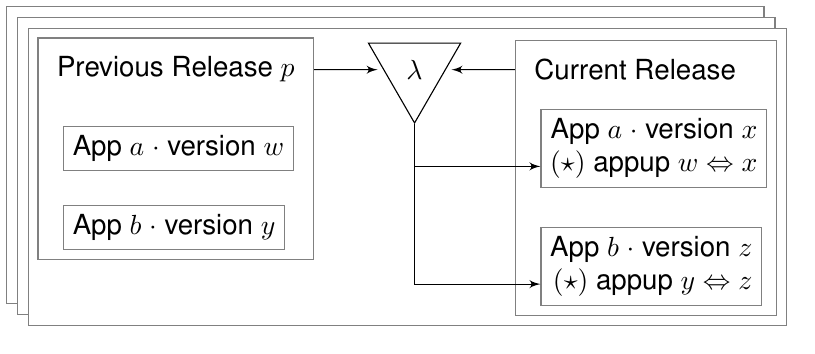
\begin{tikzpicture}[
        >=latex',
        release/.style={},
        app/.style={rectangle, draw=black!50, anchor=west},
        generator/.style={
          draw,
          shape border rotate=180,
          regular polygon,
          regular polygon sides=3,
          align=center
        }
      ]
        \pgfdeclarelayer{background}
        \pgfdeclarelayer{foreground}
        \pgfsetlayers{background,main,foreground}

        \node [release] (prev1) {Previous Release $p$};
        \node [below=of prev1.west, app, xshift=2mm] (prev1_app1) {App $a$ $\cdot$ version $w$};
        \node [below=of prev1_app1.west, app] (prev1_app2) {App $b$ $\cdot$ version $y$};
        \node [draw=black!50, fit={
          (prev1) (prev1_app1) (prev1_app2)
        }] (prev1_box) {};

        \node [generator, right=of prev1] (appup_generator) {$\lambda$};

        \node [release, right=of appup_generator] (curr1) {Current Release};
        \node [below=of curr1.west, app, xshift=2mm, align=right] (curr1_app1) {App $a$ $\cdot$ version $x$\\$(\star)$ \acrshort{appup} $w\Leftrightarrow{}x$};
        \node [below=of curr1_app1.west, app, yshift=-5mm, align=right] (curr1_app2) {App $b$ $\cdot$ version $z$\\$(\star)$ \acrshort{appup} $y\Leftrightarrow{}z$};
        \node [draw=black!50, fit={
          (curr1) (curr1_app1) (curr1_app2)
        }] (curr1_box) {};

        \path[draw,->,shorten >=2pt] (prev1 -| prev1_box.east) to (appup_generator);
        \path[draw,->,shorten >=2pt] (curr1 -| curr1_box.west) to (appup_generator);

        \path[draw,->] (appup_generator.south) |- (curr1_app1.189);
        \path[draw,->] (appup_generator.south) |- (curr1_app2.189);

        \begin{pgfonlayer}{background}
          \node [draw=black!50, fit={
            (prev1_box) (curr1_box)
          }, fill=white, double copy shadow={shadow xshift=-4pt,
          shadow yshift=4pt, fill=white, draw}] (generation) {};
        \end{pgfonlayer}

      \end{tikzpicture}
    }{\caption{\acrfull{appup} generation.}\label{fig:appup_gen}}
  \end{subfloatrow}
  \vspace{40pt} \\
  \begin{subfloatrow}
    \ffigbox[\textwidth]{
      \centering
      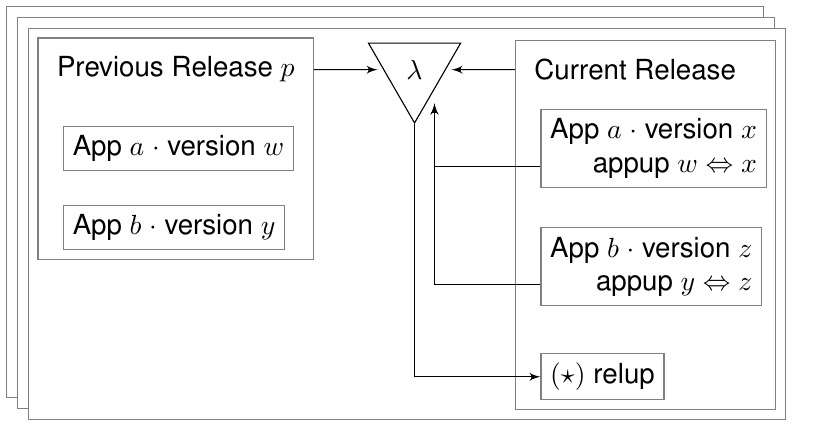
\begin{tikzpicture}[
        >=latex',
        release/.style={},
        app/.style={rectangle, draw=black!50, anchor=west},
        generator/.style={
          draw,
          shape border rotate=180,
          regular polygon,
          regular polygon sides=3,
          align=center
        }
      ]
        \pgfdeclarelayer{background}
        \pgfdeclarelayer{foreground}
        \pgfsetlayers{background,main,foreground}

        \node [release] (prev1) {Previous Release $p$};
        \node [below=of prev1.west, app, xshift=2mm] (prev1_app1) {App $a$ $\cdot$ version $w$};
        \node [below=of prev1_app1.west, app] (prev1_app2) {App $b$ $\cdot$ version $y$};
        \node [draw=black!50, fit={
          (prev1) (prev1_app1) (prev1_app2)
        }] (prev1_box) {};

        \node [generator, right=of prev1] (appup_generator) {$\lambda$};

        \node [release, right=of appup_generator] (curr1) {Current Release};
        \node [below=of curr1.west, app, xshift=2mm, align=right] (curr1_app1) {App $a$ $\cdot$ version $x$\\\acrshort{appup} $w\Leftrightarrow{}x$};
        \node [below=of curr1_app1.west, app, yshift=-5mm, align=right] (curr1_app2) {App $b$ $\cdot$ version $z$\\\acrshort{appup} $y\Leftrightarrow{}z$};
        \node [below=of curr1_app2.west, app, yshift=-4mm] (relup) {$(\star)$ \acrshort{relup}};
        \node [draw=black!50, fit={
          (curr1) (curr1_app1) (curr1_app2) (relup)
        }] (curr1_box) {};

        \path[draw,->,shorten >=2pt] (prev1 -| prev1_box.east) to (appup_generator);
        \path[draw,->,shorten >=2pt] (curr1 -| curr1_box.west) to (appup_generator);


        \path[draw,->,shorten >=5pt] (curr1_app1.189) -| (appup_generator.south east);
        \path[draw,->,shorten >=5pt] (curr1_app2.189) -| (appup_generator.south east);

        \path[draw,->] (appup_generator.south) |- (relup);

        \begin{pgfonlayer}{background}
          \node [draw=black!50, fit={
            (prev1_box) (curr1_box)
          }, fill=white, double copy shadow={shadow xshift=-4pt,
          shadow yshift=4pt, fill=white, draw}] (generation) {};
        \end{pgfonlayer}

      \end{tikzpicture}
    }{
      \caption{
        \acrfull{relup} generation.}\label{fig:relup_gen}
    }
  \end{subfloatrow}
  \vspace{6pt}
  \begin{center}
    $(\star)$ denotes new files.

    $\lambda$ is the appup generator.
  \end{center}
  \vspace{20pt}
  \begin{subfloatrow}
    \ffigbox[\textwidth]{
      \setlength{\tabcolsep}{2pt}
      \renewcommand{\arraystretch}{1.3}
      \begin{tabular}{ r r c r r }
        $p[a]$: & $w\;\Leftrightarrow\;{}x$ &
          \multirow{4}{*}{
            \hspace{10pt}
            \large{$\rightarrow$}
            \hspace{10pt}
          }& \\
        $q[a]$: & $g\;\Leftrightarrow\;{}x$ & &
          $a$: & $(w|g)\;\Leftrightarrow\;{}x$ \\
        $p[b]$: & $y\;\Leftrightarrow\;{}z$ & &
          $b$: & $(y|h)\;\Leftrightarrow\;{}z$ \\
        $q[b]$: & $h\;\Leftrightarrow\;{}z$ & & \\
      \end{tabular}
    }{\caption{Combination of upgrade instructions.}\label{fig:instruction_merge}}
  \end{subfloatrow}
  \vspace{10pt} \\
}{\caption{Generating upgrade instructions.}}

\cleardoublepage
\subsubsection{Release Upgrade Instructions} Erlang/\acrshort{otp} ships with the \acrfull{sasl} application that includes a function to assemble multiple high-level \acrfull{appup} files into a single low-level \acrfull{relup} file. Additionally, \lstinline|rebar3| wraps the \acrshort{relup} assembler in a convenience command that takes care to correctly set up the environment before invoking the generator. While the bare \acrshort{relup} generator handles multiple previous releases directly, the wrapper provided by \lstinline|rebar3| is in fact another wrapper over \lstinline|relx|, which finally calls \acrshort{sasl}. At one point in this chain, the ability to handle multiple previous releases is lost, so the tool has to engage a similar technique as the one used for generating \acrshort{appup}s. For each previous release, the current project is cloned, because in addition to the \acrshort{appup} files, the \acrshort{relup} generator also needs access to the previous release resource file and expects previous versions of the applications inside the application directory of the current release, so the previous applications are copied to the clone of the current project. The \acrshort{relup} generator is invoked to produce a \lstinline|relup| file inside the clone of the current project. Note that in contrast to \acrshort{appup} generation, which produces one instructions file for each application contained within the release, this time the application's \acrshort{appup}s are combined into a single \acrshort{relup} file as depicted in figure~\ref{fig:relup_gen}. Note that each run of the \acrshort{relup} generator must happen between exactly two releases, and that one \acrshort{relup} file is generated for each previous release, containing only the instructions to upgrade from that specific previous releasae. The resulting \acrshort{relup}s are again collected and the temporary clones are deleted. The \acrshort{relup} files have almost the same structure as the \acrshort{appup} files, so the collected instructions can be merged in the same way. The resulting single \acrshort{relup} file that now knows how to upgrade from any previous release to the current release is output to the primary working copy of the current project.

\paragraph{Packaging and storing the release.} With a final, merged \acrshort{relup} file in place, the release is ready to be packaged as a gzip-compressed tarball (\lstinline|*.tar.gz|), which contains everything needed to start a \emph{target system} from scratch, or to hot upgrade a node running any of the versions of any branches that were present in the store when the build process was started. The resulting tarball artifact is sent to one of the builder's store backends: local or remote. The local backend saves the artifact to the host's file system and is meant for testing. The recommended backend to use is the remote one, which uploads the release artifact to a central store.

\cleardoublepage
\subsection{Store}

The store is a minimal \acrshort{http} server that stores release artifacts. It handles uploading and downloading of versioned artifacts, and differentiates multiple projects and machine architectures. It is implemented in Erlang on top of the \emph{Cowboy} \acrshort{http} server application. The store interface comprises just four functions: \lstinline|put| for uploading, \lstinline|get| for downloading, \lstinline|versions| for querying the stored versions and branches of a project, and \lstinline|delete| for purging artifacts. The \acrshort{http} \acrfull{api} aims to follow a \acrfull{rest} architecture. There are two resources provided, one mapping to release tarballs (figures~\ref{fig:api_singlea},~\ref{fig:api_singleb}) that handles uploading, downloading and purging; and one mapping to the notion of a project to allow querying the stored versions and the branches to which the versions belong (figure~\ref{fig:api_list}).

Both resources expect the \acrshort{http} Basic Authentification header, and validate the given credentials against a configurable value. Metadata is returned in binary encoded \acrfull{etf}. Release artifacts are currently stored on the store server's file system.

\ffigbox[\textwidth]{
  \vspace{25pt}
  \begin{subfloatrow}
    \ffigbox[\textwidth]{
      \vspace{13pt}
      \setstackgap{S}{6pt}
      $\langle$ \stackanchor{\lstinline|GET|}{\lstinline|POST|} $\rangle$
      \hspace{0.3em}
      \lstinline|/|$\langle$\emph{project name}$\rangle$\lstinline|/|release\lstinline|/|$\langle$\emph{architecture}$\rangle$\lstinline|/|$\langle$\emph{branch}$\rangle$\lstinline|/|$\langle$\emph{version}$\rangle$
      \vspace{8pt}

      Content Type: \lstinline|application/gzip|

    }{\caption{Downloading or uploading a single artifact.}\label{fig:api_singlea}}
  \end{subfloatrow}
  \vspace{35pt} \\
  \begin{subfloatrow}
    \ffigbox[\textwidth]{
      \vspace{13pt}
      \lstinline|DELETE|
      \hspace{0.3em}
      \lstinline|/|$\langle$\emph{project name}$\rangle$\lstinline|/|release\lstinline|/|$\langle$\emph{architecture}$\rangle$\lstinline|/|$\langle$\emph{branch}$\rangle$\lstinline|/|$\langle$\emph{version}$\rangle$
      \vspace{8pt}
    }{\caption{Purging a single artifact.}\label{fig:api_singleb}}
  \end{subfloatrow}
  \vspace{35pt} \\
  \begin{subfloatrow}
    \ffigbox[\textwidth]{
      \lstinline|GET|
      \hspace{0.3em}
      \lstinline|/|$\langle$\emph{project name}$\rangle$\lstinline|/|release\lstinline|/|$\langle$\emph{architecture}$\rangle$

      \vspace{8pt}

      Content Type: \lstinline|application/erlang|

      \acrfull{etf}

    }{\caption{Querying available versions and branches.}\label{fig:api_list}}
  \end{subfloatrow}
  \vspace{25pt} \\
}{\caption{\acrshort{rest} \acrshort{api} of the store component.}}

\cleardoublepage
\section{Discussion}

The following two sections qualitatively review the contribution with respect to the stated goals, and expose limitations of the current implementation as well as discuss flaws inherent to the design.

\subsection{Advantages}

\paragraph{One time setup.} The tool is meant to be used as part of a \acrfull{ci} pipeline. Invoking a single command generates a deployable artifact from a checkout of the code base. Version identifiers are constructed out of commit timestamps and hashes, and \acrfull{appup} are generated on a best-effort basis. Previous releases are fetched from a central store, where the newly generated release artifact is uploaded to.

\paragraph{.} The \acrshort{cli} build tool is installed with a single command that does not need super user permissions, is not dependent on any specific package manager, and has no dependencies except \lstinline|curl|, \lstinline|bash| and Git––which can safely be assumed to exist on the system.

\paragraph{\acrshort{ci} support.} The tool has been shown to work on at least six common hosted \acrfull{ci} providers: \emph{Travis \acrshort{ci}, Codeship, Circle \acrshort{ci}, Wercker, Semaphore,} and \emph{Shippable}. Build run time and setup effort are comparable across providers.

\paragraph{Declarative.} The command to start a build is always the same, there are no flags or parameters. All settings such as authentification credentials for the store, or the version of Erlang/Elixir to use are passed to the tool via environment variables. The build process requires no interaction.

\paragraph{Single cache.}  Instead of having to configure and maintain multiple cache paths that may change in the future, the cache locations of various tools used within the build process are consolidated inside one directory.

\paragraph{Normalized environment.} The tool detects whether it is being run directly on a \acrshort{vm}, in which case it attempts to normalize the environment by starting a container. Nevertheless, the tool aims to be well behaved with respect to its environment.

\paragraph{Read only.} The tool never modifies the original project folder. All operations happen on temporary copies, preferably on a \acrshort{ram} disk, and the only artifact produced by a build run is a single deployable tarball. The compressed release artifact is either directly uploaded to a remote store, or written to the file system as specified by an environment variable.

% --
\cleardoublepage
\subsection{Limitations}

\paragraph{Installer.}\label{sec:curlpipesh} Distributing the \acrshort{cli} tool by downloading a script and piping it to the shell, thereby immediately executing its arbitrary contents may appear to be unsafe. Yet there is currently no simpler solution. The content delivery network that serves the installer script is configured to only accept connections over \acrshort{http}S, and \lstinline|curl| verifies the validity of the certificate. The installer is wrapped in a shell function to guard against executing a partially downloaded script. Besides, those concerned about the security implications can circumvent the installer by manually cloning a vetted checkout of the \acrshort{cli} repository.

\paragraph{Linux only.} Since the build process always runs inside a Linux container, the resulting release artifact only runs on Linux systems as well. Note that the \acrshort{cli} tool itself may be invoked on other \acrshort{os}s where Docker is supported, such as macOS, as the Docker client will then transparently run the container on a virtualized Linux kernel.~\cite{docker:docs} Consequently, the built release still only supports Linux.

\paragraph{Minimal customization.} The tool aims to cover only the most common default project configurations. This implies that all configuration files for the respective tools are in their standard locations, and that the project is set up like the scaffolding generated by the \lstinline|beamup new| command. Advanced features of the build tools such as build profiles, native dependencies, or multiple releases are not supported.

\paragraph{Already containerized pipeline.} All but one of the tested \acrshort{ci} providers run the build inside a preconfigured container, with only Travis \acrshort{ci} offering the choice between a container or a \acrshort{vm}. When the container has already been started, the launcher cannot make certain optimizations. Namely, it cannot mount a \acrshort{tmpfs} \acrshort{ram} disk, or consolidate the cache folders. The tool must also assume that the correct version of Erlang/\acrshort{otp} is already installed.

\paragraph{High \acrshort{ram} or disk usage during build.}
To avoid disk thrashing and to improve performance, the tool attempts to copy the project folder onto a \acrshort{ram} scratch disk. This working copy is naively duplicated multiple times during the build process, at least twice for every upgrade from a previous release. Note that in case the \acrshort{ram} disk fills the available memory, the \acrshort{os} falls back to using swap space. Nevertheless, the builder attempts to keep the number of concurrently existing duplicates to a minimum.


\paragraph{Store is an active component.} The builder currently supports two backends for storing built artifacts. The release tarball may either be output to the local file system, or uploaded to the store, which is an active server component that must be deployed and maintained. The current feature set implies that an active store component is unnecessary, and a backend for e.g.~a simple object storage would suffice.

The \acrshort{api} and implementation of the store server is incomplete and will in the future be extended to cover additional aspects of release handling, deployment and bootstrapping of nodes.

\paragraph{Possibly unnecessary downloading of previous releases.} The tool currently downloads the entirety of all previous releases to generate upgrade instructions. An alternative would be to locally check out the previous commits to upgrade from, compile each previous release from the checked out code, and then to compare them to generate upgrade instructions, as documented by~\cite{rebar3appup}. This paper has not evaluated advantages or limitations of a local-only approach.

\paragraph{Releases contain debug information.} Expanding the point made above, the current approach might be flawed in the following way: To generate upgrade instructions from previous releases, the bytecode files needed to be compiled with included debug information. This can be used to reconstruct the Erlang source code.~\cite{doc:otp}

\paragraph{Transient network failures.} Out of 448 test runs, three failed. Two failed attempts to download a dependency could have been caught and retried by the build tool. Retrying on network failures should arguably be a concern of the lower-level tool which initiated the request, yet a similar case could be made for handling them in the proposed tool. Unstable builds interfere with the \acrshort{ci} workflow, thus only irrecoverable errors should bubble up to affect the \acrshort{ci} build status.

\paragraph{Machine architecture support.} Though untested, the tool should be able to run on various machine architectures, and produce releases runnable on all of the architectures for which official Erlang/OTP Docker images~\cite{docker:erlang} are available: \lstinline|amd64|, \lstinline|arm32v7|, \lstinline|arm64v8|, \lstinline|i386|, \lstinline|ppc64le|, \lstinline|s390x|. However, the tool has not been tested on any machine architectures except \lstinline|amd64|. There is also no cross compilation support, nor is it expected that dependencies in the form of Erlang \acrfull{nif}~\cite{doc:otp} can be part of projects built with the proposed tool.

\paragraph{Best-effort \acrshort{appup} generation.} The build tool trades full control over the build process for hands-off operation. In certain situations with complicated dependencies between modules, processes, or even nodes the algorithm by~\cite{rebar3appup}
for generating \acrfull{appup} files may produce incorrect results, leading to failed \acrshort{dsu} attempts. However, if such situations are known beforehand, e.g.~through careful testing of upgrades, the developer may add handwritten \acrshort{appup} template files (\lstinline|*.appup.src|) to the respective applications to guide the algorithm.

\paragraph{No eviction of old releases.} The current implementation of the build tool never deletes old artifacts from the store. It also always fetches all previously stored releases to build upgrades from, leading to increasingly long build times.

\cleardoublepage
\section{Future Work}

The implementation of the node agent described in this work is a proof of concept. Further work is needed before the pipeline is fit be used in a production setting.

Every release artifact must include a full copy of the \acrshort{erts}, and the node agent always downloads the full package before each upgrade. In order to stay compatible with other \acrshort{otp} tooling while optimizing for bandwidth, the store may rebuild the generated tarball using a packing algorithm that allows efficient binary diffing of compressed artifacts.
Large deployments may also benefit from a peer-to-peer release distribution mechanism, using e.g. BitTorrent.

Configuration management was only touched upon lightly in this work and relies on files baked into the release artifacts. Since such configuration often includes sensitive data, more research is needed on how to merge the notion of \acrshort{dsu} with changing configuration at the same time; while ideally separating the delivery of software from delivery of its configuration. A node should only require a one-time setup phase where it is assigned an immutable, unique identifier. The node then uses this token to dynamically fetch all other configuration from an external service, authenticate with the store, and download releases.

While Erlang/OTP provides a way to synchronize the upgrade process between distributed nodes, there are no mechanisms for synchronizing rollback. If an upgrade fails on some of the machines and causes them to reboot with the previous release, the distributed system is left running inconsistent versions. Node agents running next to the operational nodes could form an overlay network to decide whether to perform rollbacks on all other nodes in this case.

Further research into upgrade safeness properties of Erlang/OTP systems is needed. Static linter tools could help catch common mistakes such as infinitely blocking receive clauses. To identify possibly breaking changes in record definitions for example, a more sophisticated heuristic code analysis tool may take a module's history from source control into account. Finally, online instrumentation on running nodes may provide a notion of transparently versioned message passing between Erlang processes, and help in determining the point in time when it is safe to remove deprecated message handling code.

% --
\cleardoublepage
\section{Conclusion}

This work has shown how the manual steps of deploying and upgrading an Erlang/\acrshort{otp} node can be automated. The contribution is an extension to the \acrshort{cli} tool \emph{BeamUp} to set up an Erlang node with one command that subscribes to a central release store and continuously pulls and deploys \acrshort{otp} Releases using \acrshort{dsu}.




To provide a clean and reproducible build environment, the tool transparently compiles the project inside a container. An evaluation has demonstrated that the tool works correctly and with comparable performance on major hosted \acrshort{ci} platforms.


\renewcommand{\listtablename}{Tables}

\listoffigures
\begingroup
\let\clearpage\relax
\listoftables
\endgroup
\begingroup
\let\clearpage\relax
\lstlistoflistings
\endgroup


\bibliography{lit}
\bibliographystyle{alpha}

\end{document}
